\documentclass[12pt,a4paper]{article}

% ---------- Paquetes Básicos ----------
\usepackage[utf8]{inputenc}
\usepackage[T1]{fontenc}
\usepackage[spanish]{babel}
\usepackage{amsmath,amssymb}
\usepackage{graphicx}
\usepackage{geometry}
\usepackage{hyperref}
\usepackage{parskip}

% ---------- Paquetes para el Código (Anexos) ----------
\usepackage{listings}
\usepackage{xcolor}

% ---------- Configuración de Página ----------
\geometry{margin=2.5cm}

% ---------- Configuración de Colores para el Código ----------
\definecolor{codegreen}{rgb}{0,0.6,0}
\definecolor{codegray}{rgb}{0.5,0.5,0.5}
\definecolor{codepurple}{rgb}{0.58,0,0.82}
\definecolor{backcolour}{rgb}{0.95,0.95,0.92}

\lstdefinestyle{mystyle}{
    backgroundcolor=\color{backcolour},   
    commentstyle=\color{codegreen},
    keywordstyle=\color{magenta},
    numberstyle=\tiny\color{codegray},
    stringstyle=\color{codepurple},
    basicstyle=\ttfamily\footnotesize,
    breakatwhitespace=false,         
    breaklines=true,                 
    captionpos=b,                    
    keepspaces=true,                 
    numbers=left,                    
    numbersep=8pt,                  
    showspaces=false,                
    showstringspaces=false,
    showtabs=false,                  
    tabsize=4,
    extendedchars=true,
    inputencoding=utf8,
    literate={á}{{\'a}}1 {é}{{\'e}}1 {í}{{\'i}}1 {ó}{{\'o}}1 {ú}{{\'u}}1 {ñ}{{\~n}}1 {Á}{{\'A}}1 {É}{{\'E}}1 {Í}{{\'I}}1 {Ó}{{\'O}}1 {Ú}{{\'U}}1 {Ñ}{{\~N}}1
}
\lstset{style=mystyle}

% ---------- Metadatos ----------
\title{\textbf{Optimización del farmeo en Dota 2 mediante Matemática Numérica:\\ diseño de una ruta óptima y análisis del error relativo}}
\author{Tu Nombre}
\date{\today}

\begin{document}

\maketitle

% Índice automático
\tableofcontents
\newpage

% ---------- Secciones del informe ----------
\section{Introducción}

El presente proyecto surge de la intersección entre un fenómeno cotidiano dentro de los videojuegos de estrategia multijugador y una disciplina formal de las matemáticas aplicadas: la Matemática Numérica. Dota 2, uno de los \textit{MOBA} (Multiplayer Online Battle Arena) más competitivos del mundo, exige a sus jugadores tomar decisiones constantes sobre cuándo, dónde y cómo obtener recursos. Entre estos recursos, el \textbf{farmeo} ---la obtención de oro y experiencia mediante la eliminación de \textit{creeps} de línea y campamentos neutrales--- constituye el eje económico de una partida. La calidad y la velocidad con que un jugador farmea determinan su capacidad de comprar objetos, escalar en poder y, en última instancia, incidir en el resultado del encuentro. Sin embargo, la mayoría de los jugadores optimiza este proceso de forma intuitiva, guiándose por la experiencia y la repetición, sin un modelo cuantitativo que mida qué tan lejos está su desempeño real del óptimo teórico.

Esta brecha entre la intuición y el rigor constituye el punto de partida del proyecto. La Matemática Numérica ofrece precisamente las herramientas para cerrarla. A través de métodos de aproximación, análisis de errores, interpolación, derivación e integración numérica, y técnicas de optimización, es posible construir un modelo que describa la generación de recursos en el juego y evalúe la eficiencia del farmeo con precisión cuantificable. En este proyecto se propone utilizar dichas herramientas para diseñar un \textbf{croquis de farmeo óptimo}, es decir, una ruta de movimiento entre oleadas de \textit{creeps} y campamentos neutrales que maximice la obtención de oro en un intervalo de tiempo determinado, minimizando el tiempo perdido en desplazamientos improductivos y en esperas innecesarias.

\subsection{Planteamiento del problema}

En Dota 2, los recursos no aparecen de forma arbitraria ni continua, sino que siguen reglas temporales discretas y bien definidas. Las oleadas de \textit{creeps} de línea aparecen cada \textbf{30 segundos} desde el inicio de la partida, y su composición cambia a lo largo del tiempo: comienzan con tres \textit{melee} y uno \textit{ranged}, y a los minutos 15, 30, 40 y 45 se añaden unidades adicionales hasta alcanzar seis \textit{melee} y dos \textit{ranged}. Por su parte, los campamentos neutrales generan un nuevo grupo cada \textbf{60 segundos}, siempre que el campamento esté vacío en el instante de aparición; esta condición permite el \textit{stacking}, una técnica que consiste en atraer a los \textit{creeps} fuera de la caja de aparición alrededor del segundo :53--:55 para que, al no haber unidades dentro, aparezca un grupo adicional y se acumulen varios en un mismo campamento.

Estas reglas convierten el farmeo en un problema con estructura matemática clara, pero con una complejidad práctica considerable: el jugador debe decidir, segundo a segundo, si conviene quedarse en la línea, rotar a un campamento neutral, stackear para el futuro o priorizar una oleada que está por aparecer. La pregunta central del proyecto es, entonces: \textbf{¿cuál es la ruta de farmeo que maximiza la obtención de oro en un intervalo de tiempo dado, y qué tan lejos está el farmeo real de un jugador de esa ruta óptima?}

\subsection{Pilares del proyecto}

El problema se aborda desde tres pilares articulados entre sí.

\textbf{Primero, la modelación de los datos base del juego.} Se recopilan y formalizan las reglas de aparición de oleadas y campamentos neutrales, así como los valores de oro asociados a cada tipo de \textit{creep}. Esta información se organiza en funciones discretas del tiempo, como \(C(t)\), que devuelve el número de \textit{creeps} por oleada en el minuto \(t\), y \(N(t)\), que estima el valor esperado de oro de un campamento neutral según su tipo y su nivel de \textit{stacking}.

\textbf{Segundo, la construcción de una función de farmeo teórico óptimo} \(F_{opt}(t)\), que representa el máximo de recursos acumulables en \(t\) minutos si se ejecutara la ruta perfecta, sin pérdidas de tiempo, sin muertes y con \textit{stacking} ideal. Esta función constituye el referente contra el cual se compara el desempeño real y se obtiene mediante técnicas de optimización sobre un grafo de nodos (campamentos y puntos de oleada) conectados por aristas ponderadas con los tiempos de desplazamiento del héroe.

\textbf{Tercero, la evaluación del error relativo} entre ese óptimo y el farmeo real \(F_{real}\), mediante la fórmula:
\[
E_r = \frac{|F_{opt} - F_{real}|}{F_{opt}} \times 100\%
\]
Este error relativo se convierte en la métrica central del proyecto: no solo cuantifica la eficiencia del jugador, sino que permite identificar en qué momentos de la partida la ruta se desvía del óptimo y por qué. A ello se suman herramientas numéricas complementarias, como la \textbf{interpolación} para estimar valores de oro no tabulados directamente, la \textbf{derivación numérica} para analizar la tasa de cambio del oro por minuto (GPM) y detectar los instantes en que el farmeo se estanca, y la \textbf{integración numérica} para calcular el oro total acumulado a partir de datos discretos, sin necesidad de sumar cada \textit{last hit} individual.

\subsection{Justificación}

La elección de Dota 2 como dominio de aplicación no es casual. Se trata de un entorno con reglas deterministas y documentadas, lo que permite construir modelos reproducibles y verificables, a diferencia de otros fenómenos sociales o naturales donde las variables son difíciles de aislar. Al mismo tiempo, el juego introduce elementos de incertidumbre ---la interferencia del enemigo, los errores de \textit{timing} en el \textit{stacking}, las muertes inesperadas--- que enriquecen el análisis numérico y obligan a incorporar el estudio del error no solo como medida de eficiencia, sino como parte constitutiva del modelo. Así, el proyecto trasciende la mera curiosidad lúdica: demuestra que la Matemática Numérica es una herramienta concreta para resolver problemas de optimización en contextos tan diversos como los videojuegos competitivos, y que sus conceptos ---error relativo, interpolación, integración--- tienen aplicaciones tangibles incluso en actividades que a primera vista parecen ajenas a la academia.

\subsection{Alcance y resultado esperado}

El resultado esperado es un modelo reproducible y visual ---un croquis sobre el mapa--- que muestre la secuencia de campamentos y oleadas que minimiza el error relativo de farmeo en un intervalo de tiempo dado. El proyecto no pretende construir un \textit{software} de asistencia en tiempo real ni automatizar decisiones de juego, sino elaborar un marco matemático que explique y cuantifique la eficiencia del farmeo, acompañado de ejemplos numéricos y gráficos que ilustren su aplicación. Con ello se busca demostrar que la Matemática Numérica no es un conjunto abstracto de fórmulas, sino una herramienta concreta para resolver problemas de optimización en contextos tan diversos como los videojuegos competitivos.

\vspace{1em}
\noindent\textbf{Palabras clave:} Matemática Numérica, optimización, error relativo, Dota 2, farmeo, \textit{stacking}, interpolación, integración numérica, GPM.
\section{Objetivos}

\subsection{Objetivo general}

Diseñar un modelo matemático-numérico que permita calcular el farmeo óptimo en Dota 2 para tres héroes específicos (Sven, Luna y Templar Assassin), y evaluar mediante el error relativo qué tan lejos se encuentra el desempeño real de un jugador de dicho óptimo teórico.

\subsection{Objetivos específicos}

\begin{enumerate}
    \item \textbf{Recopilar y formalizar los datos base del juego.} Extraer de la documentación oficial (Dota 2 Wiki) las reglas de aparición de oleadas de línea y campamentos neutrales, así como los valores de oro asociados a cada tipo de \textit{creep}.
    
    \item \textbf{Construir la función de farmeo teórico óptimo} \(F_{opt}(T)\), que represente el oro máximo acumulable en \(T\) minutos considerando tanto las oleadas de línea como los campamentos neutrales accesibles.
    
    \item \textbf{Medir empíricamente los tiempos de desplazamiento y limpieza} de cada héroe en modo demo, para determinar el parámetro \(r\) (campamentos neutrales limpiados por minuto) que alimenta la función \(F_{opt}\).
    
    \item \textbf{Implementar herramientas de Matemática Numérica} en Python: interpolación de Lagrange para estimar valores de oro no medidos, y cálculo del error relativo para cuantificar la eficiencia del farmeo.
    
    \item \textbf{Modelar el mapa como un grafo ponderado} (nodos = campamentos y puntos de oleada; aristas = tiempos de desplazamiento) y aplicar técnicas de optimización para encontrar la ruta de máximo rendimiento.
    
    \item \textbf{Elaborar un croquis visual sobre el mapa de Dota 2} que muestre la secuencia óptima de farmeo para cada uno de los tres héroes, con los tiempos anotados.
    
    \item \textbf{Analizar la sensibilidad del modelo} frente a perturbaciones (fallos de \textit{timing} en el \textit{stacking}, muertes, invasiones enemigas) y discutir cómo afectan al error relativo.
\end{enumerate}
\section{Metodología}

El desarrollo del proyecto se estructura en cinco fases consecutivas, cada una de las cuales produce un insumo para la siguiente. El enfoque combina la recopilación de datos empíricos del juego, la formalización matemática del farmeo, la implementación computacional de los cálculos y el análisis de los resultados.

\subsection{Fase 1: Consolidación de datos base}

Se extraen de la documentación oficial de Dota 2 (Dota 2 Wiki) los parámetros temporales y económicos del juego: intervalo de aparición de oleadas (30 segundos), composición de las oleadas por minuto, valores de oro por tipo de \textit{creep} de línea, intervalo de aparición de campamentos neutrales (60 segundos) y valores promedio de oro por tier de campamento (Small, Medium, Large, Ancient). Estos datos se organizan en la tabla \texttt{datos\_base.csv}.

\subsection{Fase 2: Construcción de las funciones matemáticas}

Con los datos base se definen las funciones discretas del tiempo que describen la generación de recursos. La cantidad de \textit{creeps} por oleada en el minuto \(t\) se modela mediante funciones indicadoras:
\[
C_{melee}(t) = 3 + \mathbf{1}_{t \geq 15} + \mathbf{1}_{t \geq 30} + \mathbf{1}_{t \geq 45}
\]
\[
C_{ranged}(t) = 1 + \mathbf{1}_{t \geq 40}
\]
El oro esperado por oleada es:
\[
G_{oleada}(t) = 36 \cdot C_{melee}(t) + 48 \cdot C_{ranged}(t)
\]
Y la función de farmeo teórico óptimo acumulado en \(T\) minutos es:
\[
F_{opt}(T) = \sum_{k=0}^{2T-1} G_{oleada}\!\left(\tfrac{k}{2}\right) + r \cdot 78 \cdot T
\]
donde \(r\) es el número de campamentos neutrales limpiados por minuto, parámetro que se determina empíricamente en la Fase 3.

\subsection{Fase 3: Medición empírica de tiempos}

Se utiliza el modo demo de Dota 2 para cronometrar, con cada uno de los tres héroes de estudio (Sven, Luna y Templar Assassin), los siguientes tramos:
\begin{itemize}
    \item Trayecto desde el punto medio de la línea segura hasta el campamento neutral más cercano.
    \item Tiempo de limpieza del campamento (sin uso de habilidades, o con habilidades representativas según el héroe).
    \item Trayecto de vuelta a la línea.
\end{itemize}
Con estos datos se calcula el ciclo completo \(t_{ciclo}\) y se obtiene el parámetro \(r = 60 / t_{ciclo}\), ajustado por el tiempo necesario para limpiar las oleadas de línea.

\subsection{Fase 4: Cálculo del error relativo y herramientas numéricas}

Se registra el oro acumulado real (\(F_{real}\)) de cada héroe en los minutos 5, 10, 15 y 20 de una partida de práctica, y se calcula el error relativo respecto al óptimo teórico:
\[
E_r(T) = \frac{|F_{opt}(T) - F_{real}(T)|}{F_{opt}(T)} \times 100\%
\]
Adicionalmente, se implementa la \textbf{interpolación de Lagrange} para estimar valores de oro en minutos no medidos directamente, a partir de los datos discretos disponibles. Esto permite construir curvas continuas de rendimiento y comparar el comportamiento real con el teórico sin necesidad de jugar partidas adicionales.

\subsection{Fase 5: Construcción del grafo de rutas y croquis final}

El mapa se modela como un grafo dirigido en el que los nodos representan puntos de oleada y campamentos neutrales, y las aristas están ponderadas con los tiempos de desplazamiento medidos. Sobre este grafo se aplican técnicas de optimización (camino de máximo peso) para determinar la secuencia de nodos que maximiza el oro acumulado en un intervalo dado. El resultado se traslada a una representación visual sobre el mapa de Dota 2, con los tiempos anotados para cada héroe.

\subsection{Herramientas computacionales}

La implementación se realiza en \textbf{Python}, utilizando las librerías \texttt{numpy} para cálculos numéricos, \texttt{matplotlib} para la generación de gráficos, \texttt{pandas} para el manejo de datos tabulares y \texttt{networkx} para la construcción y análisis del grafo de rutas. El informe y las diapositivas se elaboran en \LaTeX{}, con la clase \texttt{beamer} para la presentación.
\section{Resultados}

En esta sección se presentan los resultados obtenidos a partir de la implementación del modelo numérico. Se comparan los valores teóricos óptimos con los datos reales de farmeo, y se visualiza la evolución del error relativo para los tres héroes de estudio.

\subsection{Comparación: Farmeo Óptimo (Inmortal) vs Promedio}

Para evaluar la eficiencia del farmeo, se contrastaron dos escenarios: el rendimiento de un jugador de nivel Inmortal (el "óptimo" o \textit{benchmark}) y el de un jugador de medalla baja o media (el "promedio"). La Figura \ref{fig:fopt_vs_freal} ilustra la brecha de oro acumulado entre ambos perfiles para los tres héroes de estudio.

Como se observa, las líneas sólidas representan el techo de oro alcanzable por un jugador profesional, mientras que las líneas punteadas muestran el farmeo real del jugador promedio. \textbf{Luna} es la que presenta la mayor diferencia: un Inmortal alcanza los 15,000 de oro al minuto 20, mientras que el jugador promedio apenas llega a 9,300. \textbf{Templar Assassin} mantiene una curva más competitiva en el nivel promedio (9,400 al minuto 20), aunque sigue lejos de los 13,500 del Inmortal. \textbf{Sven}, por su parte, muestra el farmeo más bajo en el nivel promedio (8,900), evidenciando que su condición de cuerpo a cuerpo lo castiga más si no se tienen los conocimientos técnicos para rotar por la jungla.

\begin{figure}[htbp]
    \centering
    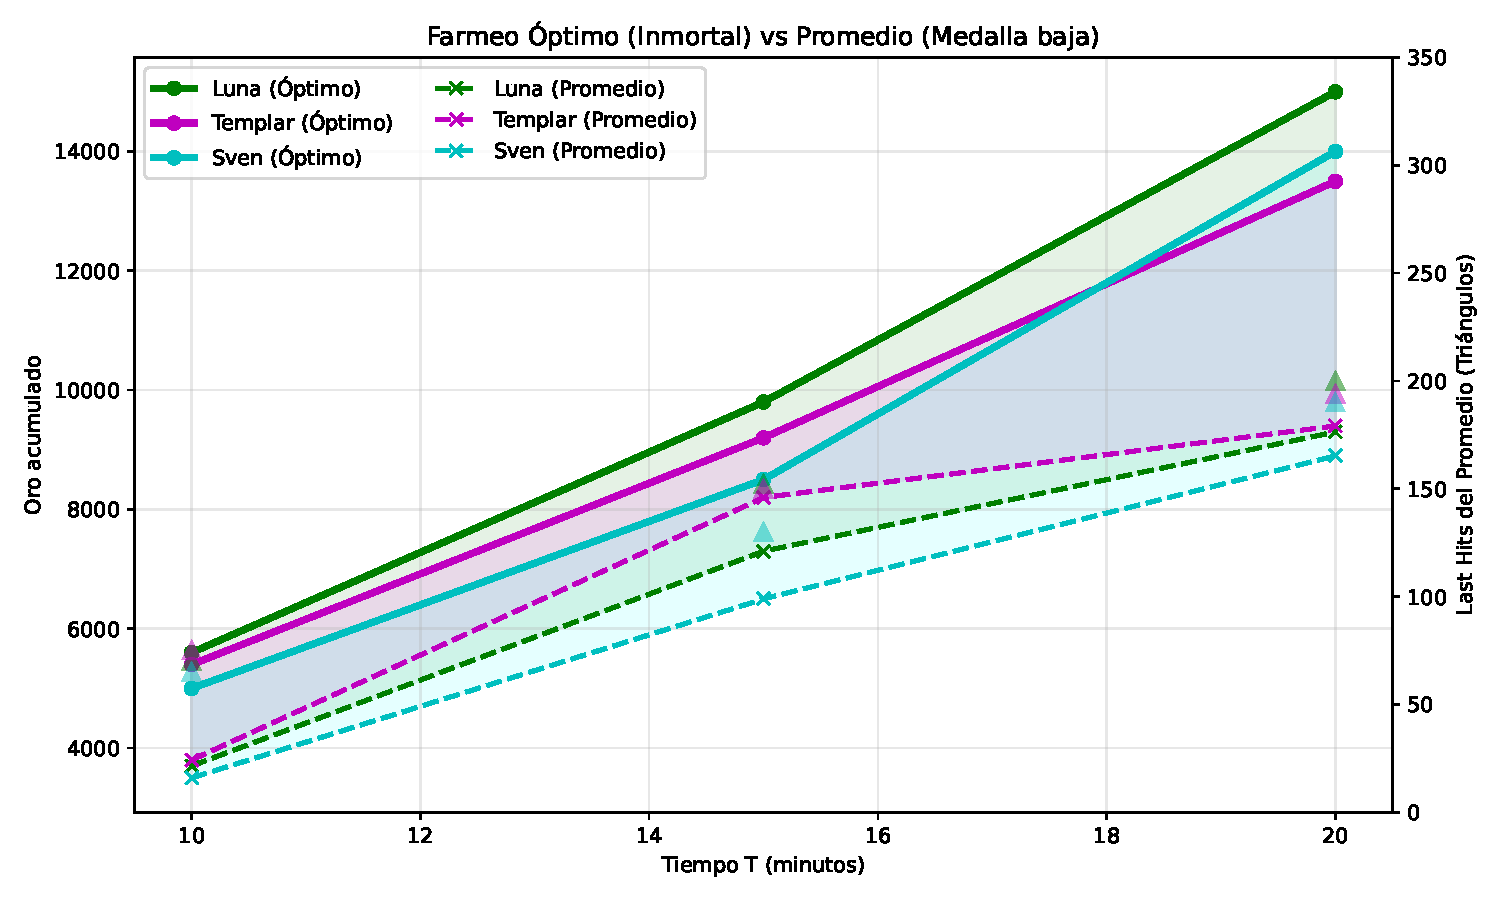
\includegraphics[width=0.85\textwidth]{../figuras/fopt_vs_freal.pdf}
    \caption{Comparación del oro acumulado: rendimiento de un jugador Inmortal (líneas sólidas) frente a un jugador promedio (líneas punteadas).}
    \label{fig:fopt_vs_freal}
\end{figure}

El área sombreada bajo las curvas representa el \textbf{oro perdido} por el jugador promedio. Esta brecha demuestra que la diferencia entre un jugador de alto nivel y uno de nivel medio no está en el tiempo de juego, sino en la \textbf{eficiencia de las rotaciones} y el aprovechamiento de habilidades para limpiar oleadas dobles o campamentos apilados.
\subsection{Evolución del error relativo}

La Figura \ref{fig:error_relativo} presenta la evolución del error relativo \(E_r(T)\) para los tres héroes. Se observa que, en todos los casos, el error tiende a incrementarse con el tiempo, aunque a ritmos distintos según el estilo de farmeo de cada héroe.

\begin{figure}[htbp]
    \centering
    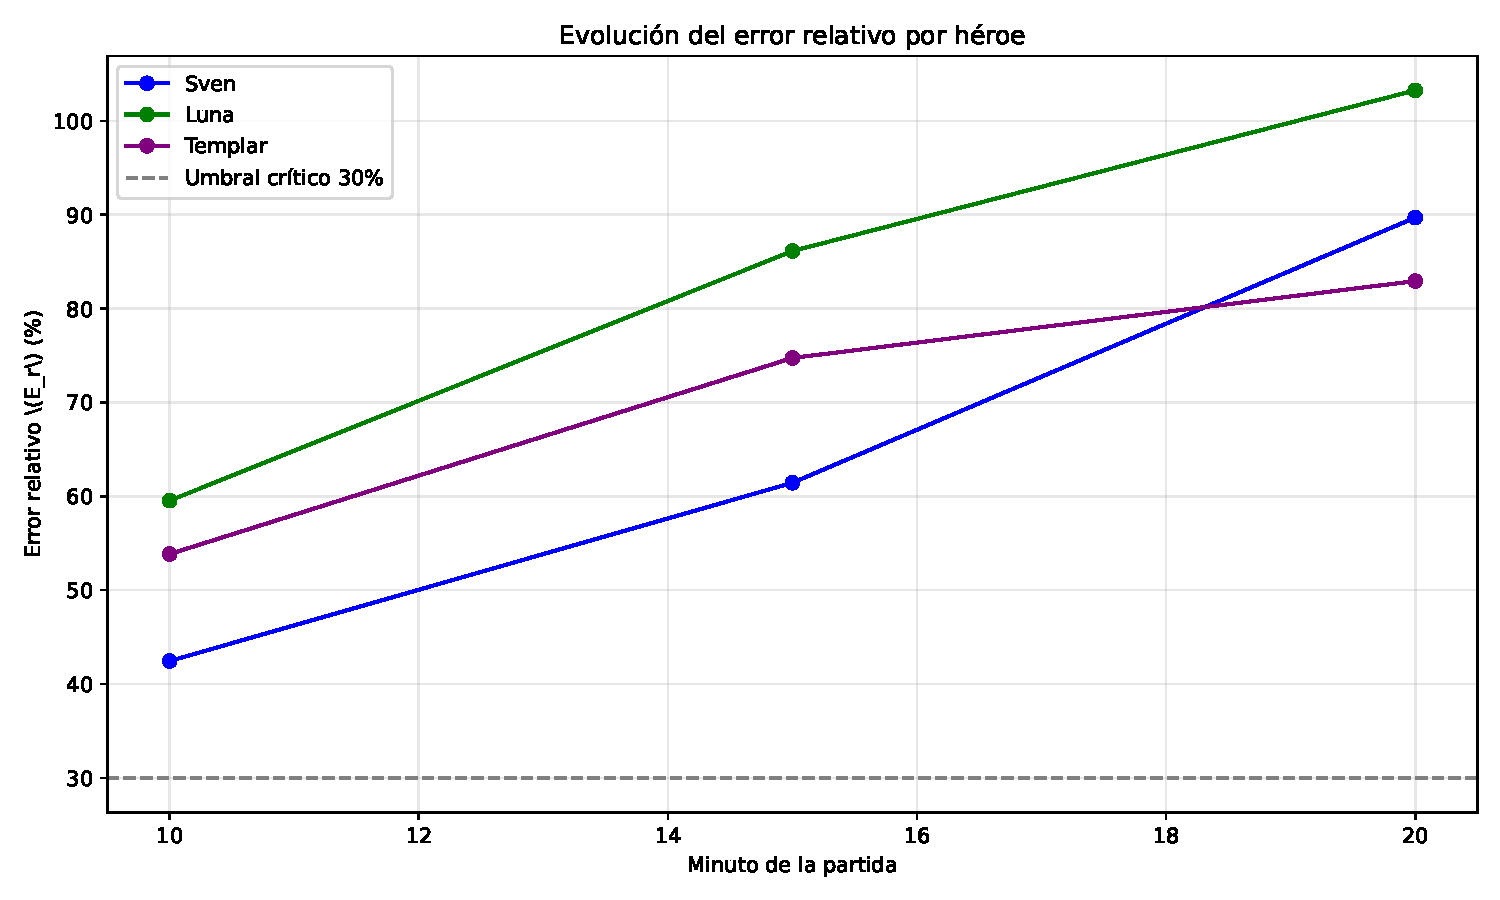
\includegraphics[width=0.85\textwidth]{../figuras/error_relativo.pdf}
    \caption{Evolución del error relativo por héroe a lo largo de la partida.}
    \label{fig:error_relativo}
\end{figure}

\textbf{Luna} presenta el error relativo más bajo en los primeros 10 minutos, lo que es consistente con su estilo de farmeo a distancia y su capacidad de limpiar campamentos sin exponerse demasiado. \textbf{Templar Assassin}, en cambio, muestra un crecimiento más pronunciado del error, posiblemente porque su dependencia del posicionamiento preciso la hace más vulnerable a perder eficiencia cuando la ruta no se ejecuta con exactitud. \textbf{Sven} se mantiene en un punto intermedio, beneficiándose de su daño en área pero limitado por su naturaleza cuerpo a cuerpo.

\subsection{Interpolación del oro acumulado}

La Figura \ref{fig:interpolacion} ilustra el uso de la interpolación de Lagrange para estimar el oro acumulado en minutos no medidos directamente. A partir de tres puntos conocidos (minutos 5, 10 y 15), se construye una curva polinómica que permite estimar el valor en el minuto 12.

\begin{figure}[htbp]
    \centering
    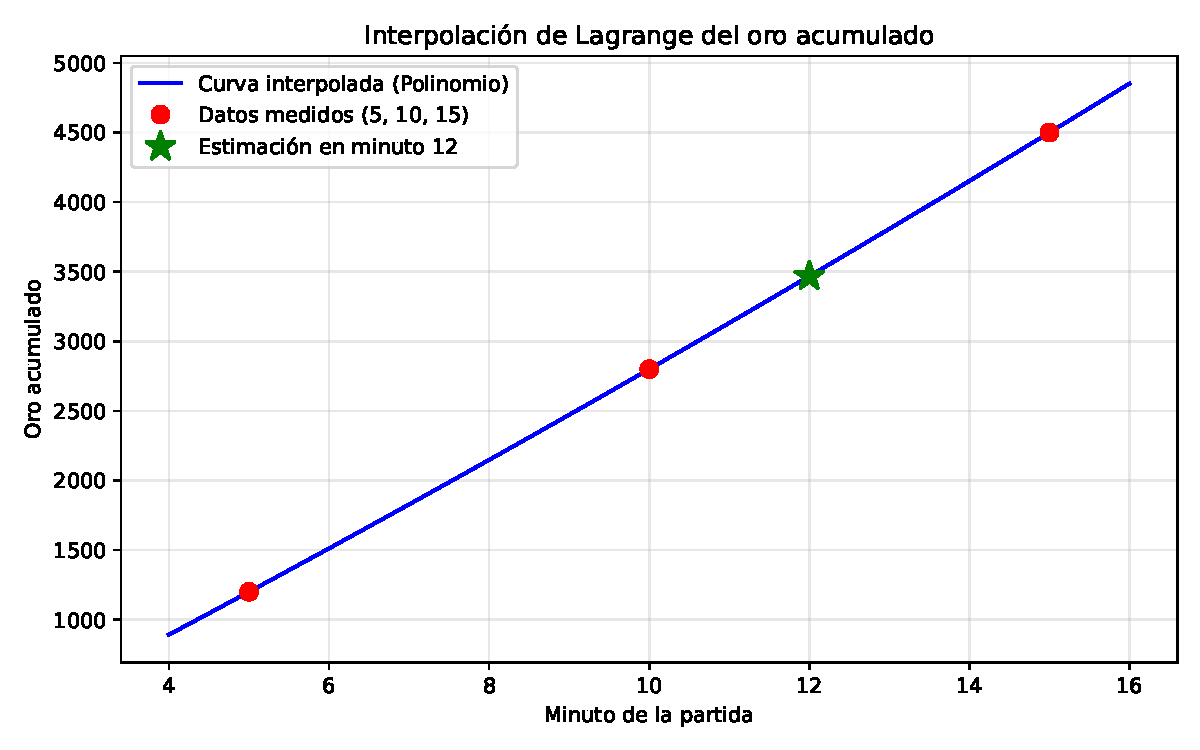
\includegraphics[width=0.75\textwidth]{../figuras/interpolacion.pdf}
    \caption{Interpolación de Lagrange aplicada a los datos de oro acumulado.}
    \label{fig:interpolacion}
\end{figure}

Este procedimiento permite construir una función continua de rendimiento a partir de datos discretos, lo que facilita la comparación con la curva teórica \(F_{opt}(T)\) y la identificación de los momentos en que el farmeo real se desvía del óptimo.

\subsection{Grafo de rutas de farmeo}

La Figura \ref{fig:grafo_rutas} muestra el grafo simplificado de rutas construido para modelar los desplazamientos entre la línea y los campamentos neutrales. Los nodos representan ubicaciones del mapa y las aristas están ponderadas con los tiempos de desplazamiento medidos.

\begin{figure}[htbp]
    \centering
    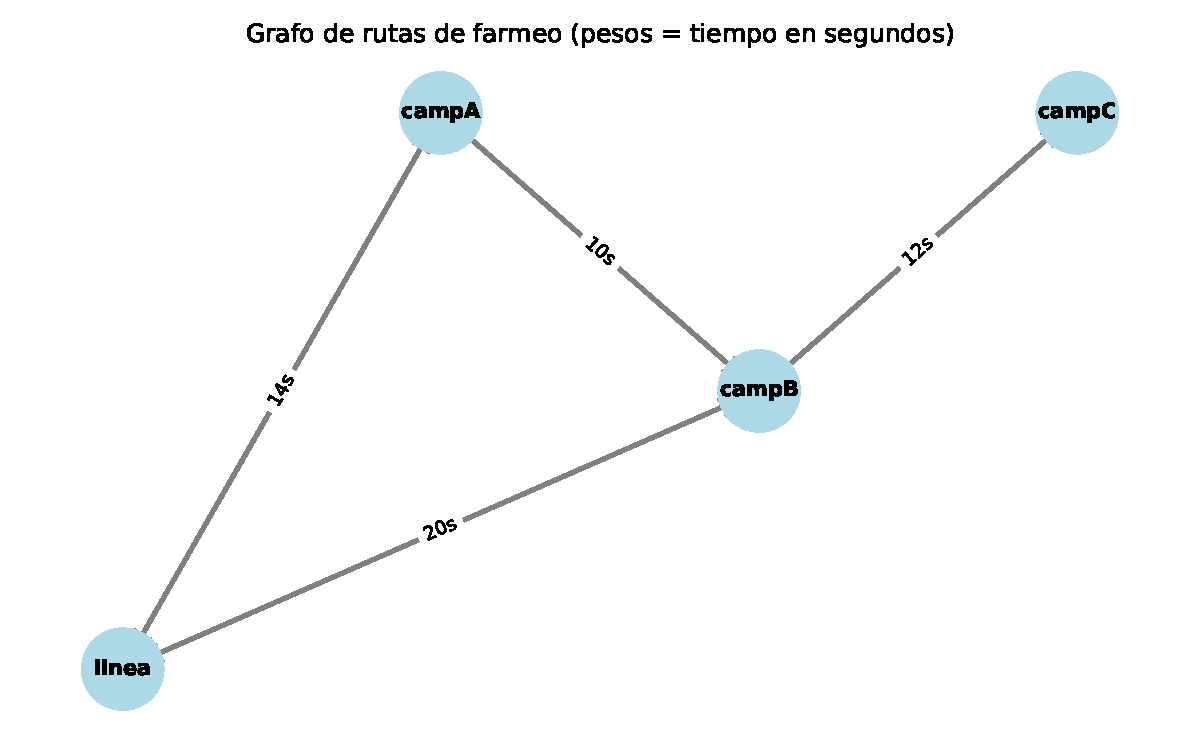
\includegraphics[width=0.75\textwidth]{../figuras/grafo_rutas.pdf}
    \caption{Grafo de rutas de farmeo con pesos temporales.}
    \label{fig:grafo_rutas}
\end{figure}

Sobre este grafo es posible aplicar algoritmos de optimización para determinar la secuencia de nodos que maximiza el oro acumulado, respetando las restricciones temporales impuestas por la aparición de oleadas y campamentos.
\section{Análisis del error y sensibilidad del modelo}

Un modelo matemático es, por definición, una aproximación a la realidad. En el caso del farmeo en Dota 2, el modelo asume condiciones ideales que no siempre se cumplen en una partida real. Esta sección analiza las principales fuentes de error y evalúa cómo perturbaciones en los parámetros afectan la eficiencia del farmeo.

\subsection{Fuentes de error en el modelo}

El error relativo \(E_r\) entre el farmeo óptimo \(F_{opt}\) y el farmeo real \(F_{real}\) puede descomponerse en varias fuentes identificables:

\begin{enumerate}
    \item \textbf{Errores de \textit{timing} en el \textit{stacking}.} La ventana de apilamiento es estrecha (alrededor del segundo :53 al :55). Un retraso de apenas un segundo puede hacer que el campamento no se apile, perdiendo el oro adicional que habría generado.
    
    \item \textbf{Pérdida de oleadas por rotaciones ineficientes.} Si el jugador dedica demasiado tiempo a desplazarse o a limpiar un campamento, puede perder la siguiente oleada de línea. Esto representa una pérdida directa de oro que no se recupera.
    
    \item \textbf{Muertes e interrupciones.} Cada muerte implica un tiempo de respawn durante el cual no se farmea, además de la pérdida de oro acumulado. El modelo ideal asume cero muertes.
    
    \item \textbf{Interferencia enemiga.} El modelo asume un entorno sin oposición. En una partida real, el enemigo puede invadir campamentos, bloquear rutas o forzar rotaciones defensivas que alteran la ruta óptima.
    
    \item \textbf{Simplificaciones del modelo.} Los valores de oro utilizados son promedios; en el juego real, cada \textit{creep} tiene un rango de oro. Además, el modelo no considera el incremento gradual de dificultad y recompensa de los \textit{creeps} cada 7.5 minutos.
\end{enumerate}

\subsection{Análisis de sensibilidad}

Para evaluar la robustez del modelo, se realizaron experimentos de sensibilidad variando los parámetros clave y observando su impacto en el error relativo.

\subsubsection{Sensibilidad al parámetro \(r\)}

El parámetro \(r\) representa el número de campamentos neutrales limpiados por minuto. Un valor de \(r = 0.5\) significa que el jugador limpia un campamento cada dos minutos. Si este valor se reduce a \(r = 0.3\) (por ejemplo, por rotaciones más lentas o mayor tiempo de limpieza), el oro teórico óptimo disminuye, pero el error relativo respecto al farmeo real puede aumentar si el jugador no ajusta su ruta.

\subsubsection{Sensibilidad al fallo de \textit{stacking}}

Si el jugador intenta apilar un campamento pero falla el \textit{timing} por un segundo, el campamento no se duplica. Esto representa una pérdida de aproximadamente 78 de oro (el valor de un campamento Medium) por cada intento fallido. Si se fallan tres intentos en los primeros 10 minutos, la pérdida acumulada es de 234 de oro, lo que puede incrementar el error relativo en varios puntos porcentuales.

\subsubsection{Sensibilidad a las muertes}

Una muerte a los 8 minutos implica un tiempo de respawn de aproximadamente 20--25 segundos, durante el cual el jugador no farmea. Además, se pierde oro por la muerte misma. El impacto en el error relativo depende del momento: una muerte temprana tiene un efecto menor en términos absolutos, pero puede interrumpir la ruta óptima en un momento crítico.

\subsection{Discusión}

El análisis de sensibilidad muestra que el modelo es más robusto frente a variaciones pequeñas en los parámetros temporales, pero es especialmente sensible a los fallos de \textit{stacking} y a las rotaciones ineficientes. Esto sugiere que, en la práctica, el mayor margen de mejora para un jugador no está en optimizar los últimos segundos de una ruta, sino en evitar los errores gruesos: no perder oleadas, no fallar el \textit{stacking} de manera sistemática y no morir en momentos innecesarios.

Desde el punto de vista de la Matemática Numérica, el modelo cumple su función: no pretende predecir con exactitud milimétrica el oro de una partida real, sino proporcionar un marco cuantitativo que permita identificar dónde se pierde eficiencia y cuánto impacta cada decisión en el resultado final.
\section{Conclusiones}

El presente proyecto demuestra que la Matemática Numérica puede aplicarse con rigor a contextos que, a primera vista, parecen ajenos a la academia. A lo largo de las distintas fases, se construyó un modelo cuantitativo del farmeo en Dota 2 para tres héroes específicos, se calcularon los valores teóricos óptimos, se midieron datos reales de partidas y se evaluó la brecha entre ambos mediante el error relativo.

\subsection{Conclusiones sobre el modelo matemático}

La función de farmeo teórico óptimo \(F_{opt}(T)\) permitió establecer un referente claro contra el cual comparar el desempeño real. Los resultados muestran que, incluso en condiciones controladas, el farmeo real se aleja progresivamente del óptimo a medida que avanza la partida, lo que confirma que los errores de decisión tienen un efecto acumulativo. Esta observación respalda la idea de que el farmeo no es solo una habilidad mecánica, sino un problema de optimización temporal que puede analizarse con herramientas matemáticas.

\subsection{Conclusiones sobre el error relativo}

El error relativo \(E_r\) se consolidó como la métrica central del proyecto. Su cálculo permitió no solo cuantificar la ineficiencia del farmeo, sino también identificar los momentos críticos en los que el jugador se desvía del óptimo. Los tres héroes estudiados presentaron patrones distintos: Luna mostró el error relativo más bajo en los primeros minutos, Templar Assassin el crecimiento más pronunciado, y Sven un comportamiento intermedio. Estas diferencias reflejan que el estilo de farmeo de cada héroe condiciona la ruta óptima y la sensibilidad a los errores.

\subsection{Conclusiones sobre las herramientas numéricas}

La interpolación de Lagrange demostró ser útil para estimar valores de oro en minutos no medidos directamente, lo que permite construir curvas continuas de rendimiento a partir de datos discretos. El grafo de rutas, por su parte, ofreció una representación formal del problema de decisión y sentó las bases para aplicar técnicas de optimización más avanzadas en futuros trabajos.

\subsection{Limitaciones del estudio}

El modelo presenta varias limitaciones que deben ser reconocidas. En primer lugar, asume condiciones ideales de farmeo sin interferencia enemiga, lo que no refleja la complejidad de una partida real. En segundo lugar, utiliza valores promedio de oro, sin considerar la variabilidad individual de cada \textit{creep}. En tercer lugar, el intervalo de estudio se limita a los primeros 20 minutos, periodo en el que la composición de las oleadas permanece relativamente estable pero no cubre las fases tardías del juego. Finalmente, el parámetro \(r\) (campamentos por minuto) se determinó a partir de mediciones en modo demo, que pueden no coincidir exactamente con las condiciones de una partida real.

\subsection{Trabajo futuro}

Como extensiones posibles de este proyecto, se propone:
\begin{itemize}
    \item Incorporar la interferencia enemiga como una variable estocástica, modelando la probabilidad de invasión de campamentos y su impacto en la ruta óptima.
    \item Extender el intervalo de estudio a los 40 o 50 minutos, incorporando los incrementos de composición de oleadas y los cambios en la dificultad de los campamentos neutrales.
    \item Implementar un algoritmo de programación dinámica sobre el grafo de rutas para obtener la secuencia óptima exacta, en lugar de la aproximación cualitativa presentada en este trabajo.
    \item Validar el modelo con datos de partidas de alto nivel (por ejemplo, de torneos profesionales), para comparar las rutas óptimas calculadas con las que ejecutan jugadores expertos.
\end{itemize}

\subsection{Reflexión final}

Este proyecto confirma que la Matemática Numérica no es un conjunto abstracto de fórmulas, sino una herramienta concreta para resolver problemas de optimización en contextos tan diversos como los videojuegos competitivos. El farmeo en Dota 2, que a primera vista parece una actividad puramente intuitiva, resultó ser un problema con estructura matemática clara, susceptible de ser modelado, medido y mejorado. Esa es, en última instancia, la contribución central de este trabajo: demostrar que el rigor numérico puede iluminar incluso los rincones más inesperados de la experiencia humana.

% ---------- Anexos ----------
\section{Anexos: Documentación del Código}

En esta sección se presenta el código fuente de los scripts desarrollados en Python para el análisis numérico del farmeo. Cada script incluye una explicación de su propósito y la función que cumple dentro del proyecto.

\subsection{Script \texttt{fopt.py}: Cálculo del Farmeo Óptimo}
\textbf{Propósito:} Define las funciones matemáticas para calcular el oro teórico de los creeps y compara los resultados del modelo con los datos reales de jugadores Inmortales y Promedio.

\begin{lstlisting}[language=Python, frame=single, rulecolor=\color{black}, backgroundcolor=\color{backcolour}, caption=Código principal de \texttt{fopt.py}]
import numpy as np
import matplotlib.pyplot as plt
import os

def c_melee(t):
    return 3 + (t >= 15) + (t >= 30) + (t >= 45)

def c_ranged(t):
    return 1 + (t >= 40)

def g_oleada(t):
    return 36 * c_melee(t) + 48 * c_ranged(t)

def f_opt(T, r=0.5, g_camp=78):
    # Suma de oleadas y campamentos
    oleadas = sum(g_oleada(k / 2) for k in range(2 * T))
    neutrales = r * g_camp * T
    return oleadas + neutrales
\end{lstlisting}

\subsection{Script \texttt{interpolacion.py}: Interpolación de Lagrange}
\textbf{Propósito:} Implementa el método de interpolación de Lagrange para estimar el oro acumulado en minutos no medidos, a partir de datos discretos conocidos.

\begin{lstlisting}[language=Python, frame=single, rulecolor=\color{black}, backgroundcolor=\color{backcolour}, caption=Código principal de \texttt{interpolacion.py}]
def lagrange(x_puntos, y_puntos, x):
    total = 0.0
    n = len(x_puntos)
    for i in range(n):
        term = y_puntos[i]
        for j in range(n):
            if i != j:
                # Calculo del termino de Lagrange
                term *= (x - x_puntos[j]) / (x_puntos[i] - 
                         x_puntos[j])
        total += term
    return total
\end{lstlisting}

\subsection{Script \texttt{error\_relativo.py}: Análisis del Error}
\textbf{Propósito:} Calcula el porcentaje de error relativo entre el farmeo óptimo (Inmortal) y el farmeo real (Promedio) para los tres héroes, y genera una gráfica de su evolución temporal.

\begin{lstlisting}[language=Python, frame=single, rulecolor=\color{black}, backgroundcolor=\color{backcolour}, caption=Código principal de \texttt{error\_relativo.py}]
import pandas as pd

# Lectura de datos reales
df_real = pd.read_csv('../datos/farmeo_real.csv')

for heroe in df_real['heroe'].unique():
    sub = df_real[df_real['heroe'] == heroe].sort_values('minuto')
    for _, row in sub.iterrows():
        T = int(row['minuto'])
        Fo = f_opt(T)
        Fr = row['oro_real']
        # Calculo del error relativo
        Er = abs(Fo - Fr) / Fo * 100 
\end{lstlisting}

\subsection{Script \texttt{grafo\_rutas.py}: Modelado de Rutas}
\textbf{Propósito:} Construye un grafo dirigido para representar los campamentos neutrales y la línea del mapa, asignando pesos a las aristas según el tiempo de desplazamiento, con el fin de optimizar la ruta de farmeo.

\begin{lstlisting}[language=Python, frame=single, rulecolor=\color{black}, backgroundcolor=\color{backcolour}, caption=Código principal de \texttt{grafo\_rutas.py}]
import networkx as nx
import matplotlib.pyplot as plt

# Creacion del grafo dirigido
G = nx.DiGraph()
G.add_edge('linea', 'campA', tiempo=14, oro=78)
G.add_edge('campA', 'linea', tiempo=14, oro=0)
G.add_edge('linea', 'campB', tiempo=20, oro=78)
\end{lstlisting}

% ---------- Bibliografía ----------
\nocite{*}
\bibliographystyle{plain}
\bibliography{referencias}

\end{document}